\subsection{Directed class transitions by answer correctness}

For each model, we separate labelled attempts by whole-answer correctness and count directed transitions between originally adjacent labelled sentences. Rows are source classes and columns are destination classes. Self-transitions are retained; missing labels and sampling gaps are never bridged. Each cell is the total observed count divided by the number of labelled attempts in that outcome group: equivalently, the mean per-attempt count, including zero-pair attempts. Empty-label attempts are excluded. These are counts per attempt, not row-normalized probabilities or full-trace transition estimates.

The two panels per model pool the six benchmarks and all six panels share one colour scale. Benchmark-specific counts and denominators are saved in the accompanying statistics JSON. Outcome groups differ in benchmark mix, reasoning length, and label coverage; Qwen also retains a different annotation protocol from Gemma and GPT-OSS. Differences are descriptive associations, not evidence that a transition causes correctness or a controlled comparison between models.

\begin{figure}[p]\centering
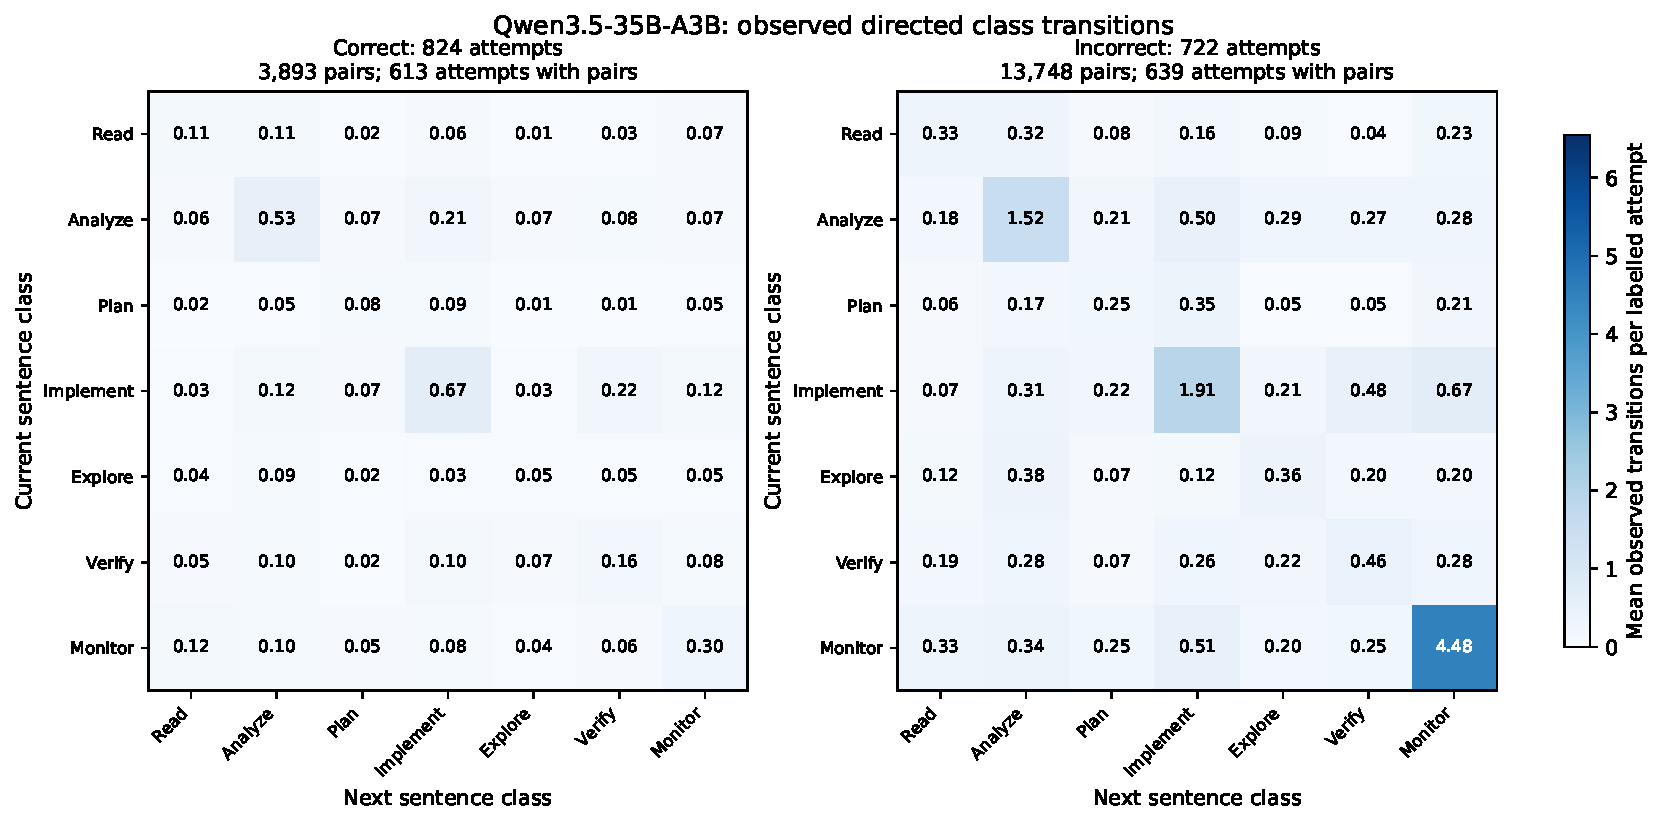
\includegraphics[width=\linewidth]{figures/qwen_class_transitions_by_correctness.pdf}
\caption{Qwen3.5-35B-A3B: directed class transitions for correct and incorrect answers. Cells show mean observed counts per labelled attempt, including self-transitions on the diagonal. Panel headings give denominators and adjacent-pair coverage; zero-pair attempts remain in the mean. The shared colour scale is identical across all three models. Sampling and population differences limit interpretation.}
\label{fig:qwen-class-transitions-by-correctness}
\Description{Two square heatmaps show directed class transition counts, split by answer correctness.}
\end{figure}

\begin{figure}[p]\centering
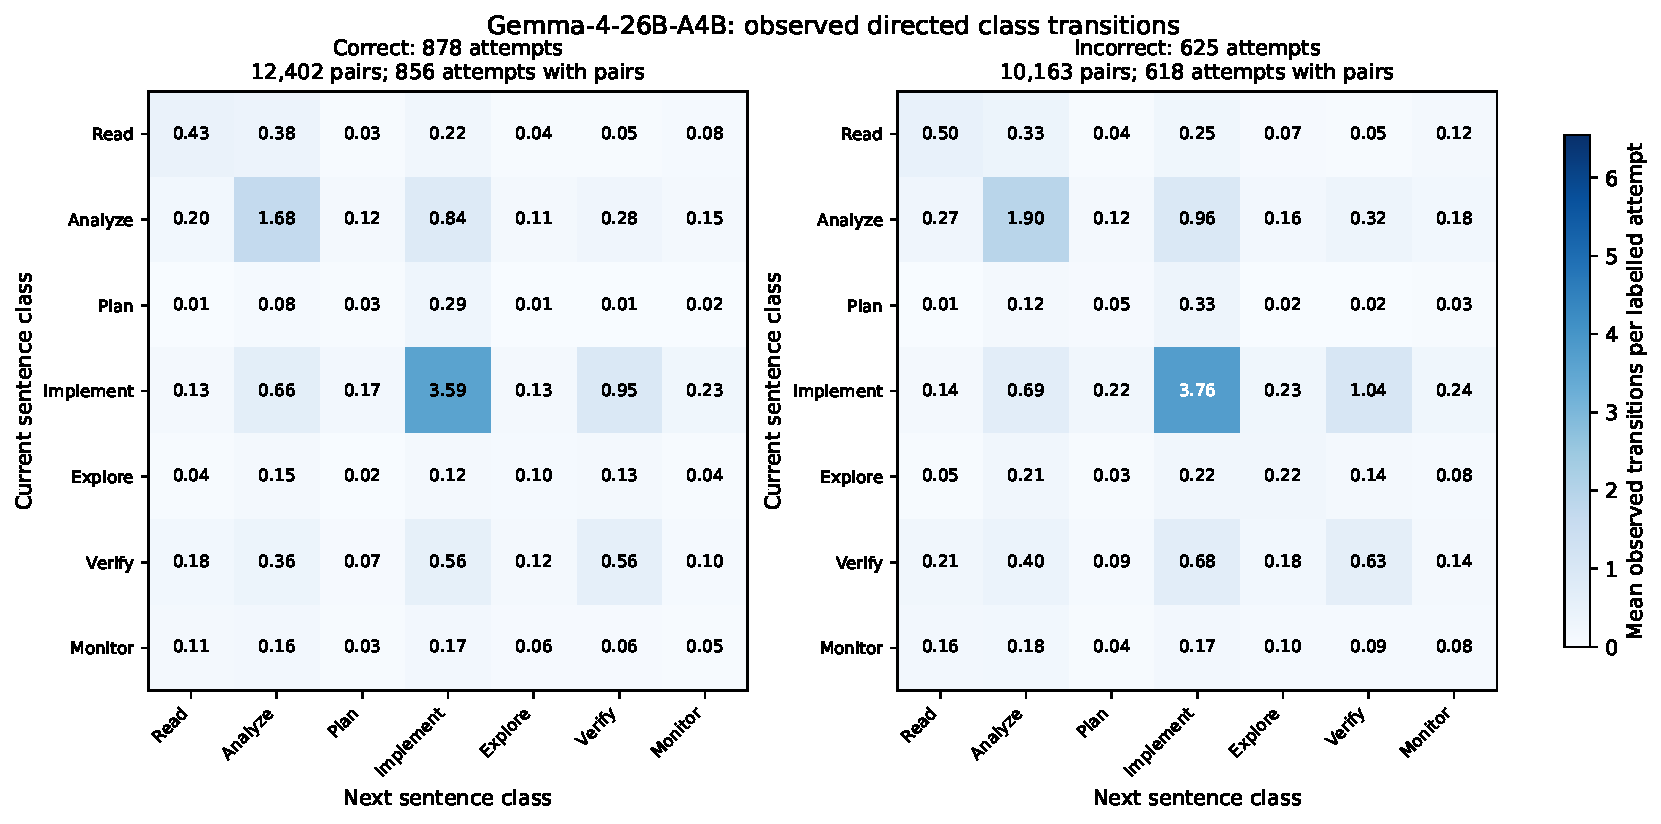
\includegraphics[width=\linewidth]{figures/gemma_class_transitions_by_correctness.pdf}
\caption{Gemma-4-26B-A4B: directed class transitions for correct and incorrect answers. Cells show mean observed counts per labelled attempt, including self-transitions on the diagonal. Panel headings give denominators and adjacent-pair coverage; zero-pair attempts remain in the mean. The shared colour scale is identical across all three models. Sampling and population differences limit interpretation.}
\label{fig:gemma-class-transitions-by-correctness}
\Description{Two square heatmaps show directed class transition counts, split by answer correctness.}
\end{figure}

\begin{figure}[p]\centering
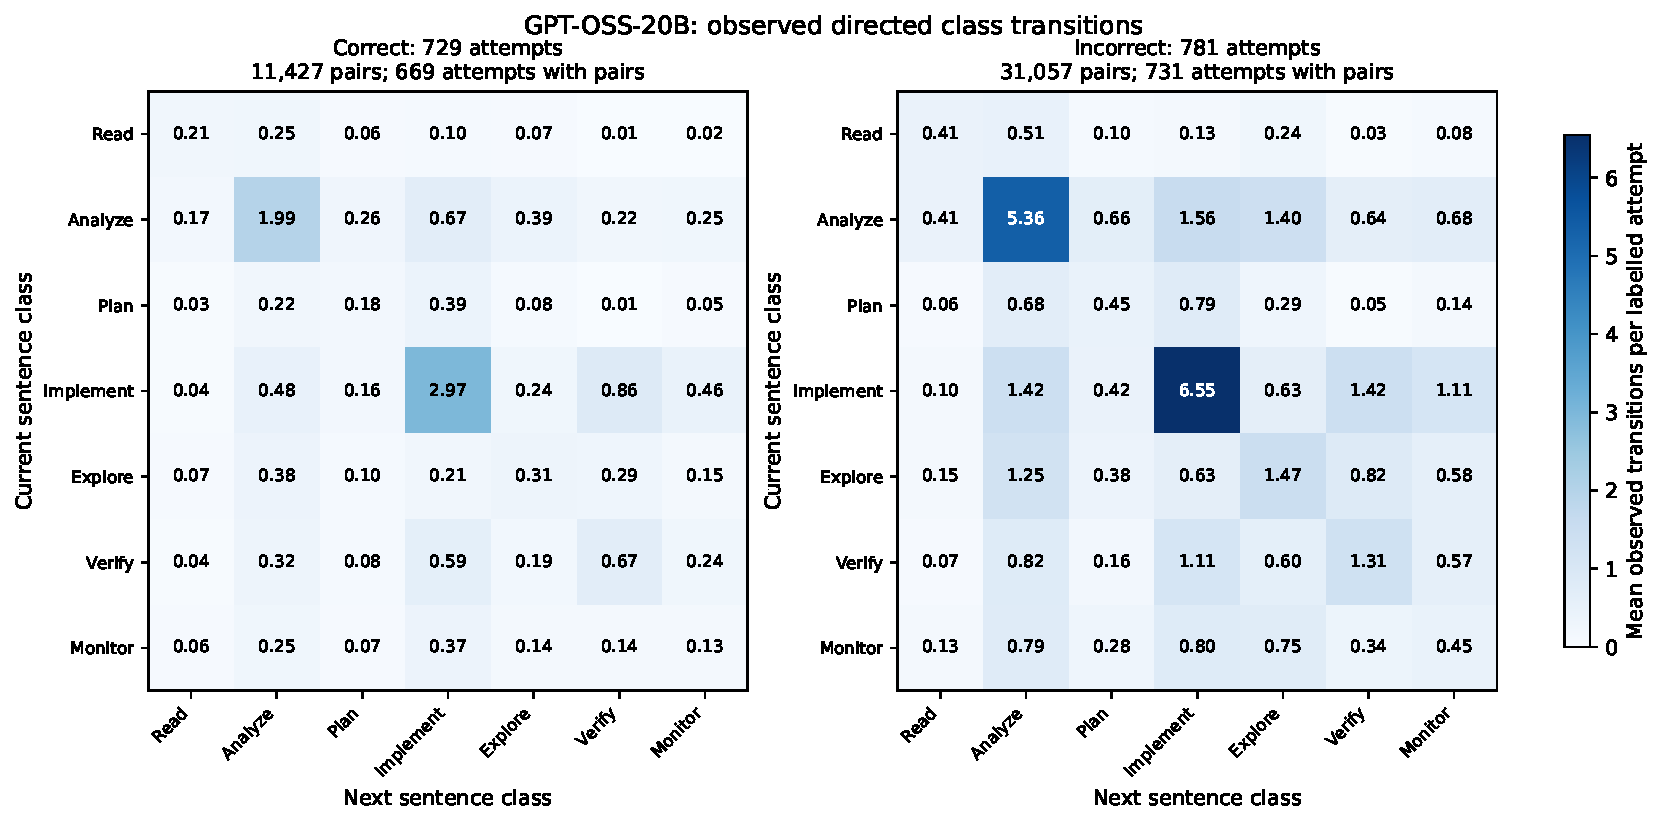
\includegraphics[width=\linewidth]{figures/gptoss_class_transitions_by_correctness.pdf}
\caption{GPT-OSS-20B: directed class transitions for correct and incorrect answers. Cells show mean observed counts per labelled attempt, including self-transitions on the diagonal. Panel headings give denominators and adjacent-pair coverage; zero-pair attempts remain in the mean. The shared colour scale is identical across all three models. Sampling and population differences limit interpretation.}
\label{fig:gptoss-class-transitions-by-correctness}
\Description{Two square heatmaps show directed class transition counts, split by answer correctness.}
\end{figure}
